\documentclass[10pt,twocolumn,letterpaper]{article} 


\usepackage{cvpr}
\usepackage{times}
\usepackage{epsfig}
\usepackage{graphicx}
\usepackage{amsmath}
\usepackage[psamsfonts]{amssymb}
\usepackage{url}

\def\RR{\mathbb{R}}
\def\NN{\mathbb{N}}
\def\xx{\mathbf{x}}
\def\ww{\mathbf{w}}
\def\aa{\mathbf{\alpha}}
\def\bb{\mathbf{\beta}}
\def\ee{\mathbf{e}}
\def\dd{\mathbf{d}}
\def\mdd{\tilde{\dd}}
\def\b{\mathcal{B}}
\def\d{\mathcal{D}}

% ------------------------------------------------------------------------ 

% Include other packages here, before hyperref.

\usepackage[pagebackref=true,breaklinks=true,letterpaper=true,colorlinks,bookmarks=false]{hyperref}
% \cvprfinalcopy % *** Uncomment this line for the final submission
\def\cvprPaperID{****} % *** Enter the CVPR Paper ID here
\def\httilde{\mbox{\tt\raisebox{-.5ex}{\symbol{126}}}}
\ifcvprfinal\pagestyle{empty}\fi

\begin{document}

% ------------------------------------------------------------------------ 

\title{Online place recognition in complex robot navigation \\
using reduced-rank support vector classification}

\author{Francesco Orabona\\
LIRA-Lab, University of Genova\\
viale F. Causa, 13, 16145 Genova, Italy\\
{\tt\small bremen@liralab.it}
% For a paper whose authors are all at the same institution, 
% omit the following lines up until the closing ``}''.
% Additional authors and addresses can be added with ``\and'', 
% just like the second author.
% To save space, use either the email address or home page, not both
\and
Second Author\\
Institution2\\
First line of institution2 address\\
{\small\url{http://www.author.org/~second}}
}

\maketitle
% \thispagestyle{empty}

% ------------------------------------------------------------------------ 

\begin{abstract}
  Real-time, online place recognition must be performed in most
  complex robot navigation tasks. In this paper we analyse the
  benefits of a novel online reduced-rank Support Vector
  Classification method in such a framework.

  In particular, we show that this method is able to retain the
  accuracy of the non-reduced method, while allowing for a reduction
  in the space requirement of up to XXXX%.
\end{abstract}

% ------------------------------------------------------------------------ 

\section{Introduction}

In a number of research fields as diverse as, e.g., bioinformatics,
data mining and robotics, it is crucial to be able to reconstruct an
unknown function given a finite set of samples and the values the
function assigns them. Given this very general problem, statistical
learning theory \cite{v-edbed-82} can tell us how close our
approximation is to the original function, and give us an indication
of how well it will work. Usually, a set of samples of the unknown
function is available, and then a machine learning algorithm is
employed to interpolate the data.

Introduced in the early 90s by Boser, Guyon and Vapnik \cite{BGV92},
\emph{Support Vector Machines} (SVMs) are a class of such algorithms
deeply rooted in statistical learning theory. As opposed to analogous
algorithms such as, e.g., artificial neural networks, they have the
main advantages that their training is guaranteed to end up in a
global solution, that they can easily work in highly dimensional,
non-linear feature spaces, and that the solution achieved is
sparse. Due to these good properties, they have been now extensively
used in, e.g., speech recognition, object classification and function
approximation with good results \cite{Cristianini00}. As opposed to
this, one of their main drawbacks is their alleged inability to cope
with large datasets, since, in their na\"\i ve version, their space
requirement is quadratic and the training time is cubic in the number
of training samples \cite{KeerthiCDC06}.

Because of this problem, there has been lately quite a lot of research
upon the sparseness of their solution. That an SVM solution is
\emph{sparse} means that usually just a few samples can account for
most of the complexity of the approximated function; in fact, SVMs can
be seen as a way of compressing data by selecting ``the most
important'' samples (\emph{support vectors}) among those in the
training set. Keeping the number of support vectors small without
losing accuracy of the solution is therefore a major issue, also since
a recent result \cite{Steinwart03} shows that the number of support
vectors grows indefinitely as more training samples are acquired and
used for training.

Following related literature, in this paper we propose a method of
selecting support vectors based upon \emph{linear independence in the
feature space}: support vectors which are linearly dependent on
already stored ones are rejected, and a smart, incremental
minimisation algorithm is employed to find the new minimum of the cost
function. The size of the kernel matrix --- basically the core of an
SVM, and the major bottleneck --- is therefore kept small. Our
experiments indicate that SVMs employing this idea, that we call
\emph{Incremental Independent Support Vector Machines} (IISVMs), do
not grow linearly with the training set, as it was the case in
\cite{Steinwart03}, but reach a limit size and then stop growing in
the case of finite-dimensional feature spaces, \emph{while keeping the
full accuracy of standard SVMs}; and that they grow dramatically less
in the infinite-dimensional case, at the price of a negligible loss in
accuracy.

The paper is structured as follows: in Section \ref{sec:bg} we
introduce some mathematical background proper to SVMs and necessary to
explain our idea; in Section \ref{sec:spars} some considerations on
the sparseness of SVM solutions are stated. In Section \ref{sec:opt}
then, we describe IISVM; in Section \ref{sec:exp} we show some
experimental results, and lastly in Section \ref{sec:concl}
conclusions are drawn and future work is outlined.

\section{Background Mathematics}
\label{sec:bg}

Assume $\{\xx_i,y_i\}_{i=1}^l$, with $\xx_i \in \RR^m$ and $y_i \in
\{-1,1\}$, is a set of samples drawn from an unknown probability
distribution. The problem is to approximate it in order to classify
more data coming from the same source to the best extent
possible. Assuming the data are linearly separable, according to the
standard approach, a \emph{separating hyperplane} in $\RR^m$ is sought
for:

\begin{equation} \label{eqn:dec}
  f(\xx) = sgn(\ww\cdot\xx + b)
\end{equation}

with $\ww \in \RR^m$ and $b \in \RR$. In this case, the hyperplane
must respect the constraints $y_i(\ww\cdot\xx_i + b)-1\geq 0$, for all
$i = 1,\ldots,l$ (from now on, this will be implicit whenever a
subscript $i$ appears free in a formula). In the general, more likely
and realistic case in which the data are not linearly separable, we
introduce $l$ slack variables $\xi_i$ and rather require that
$y_i(\ww\cdot\xx_i + b)-1+\xi_i\geq 0$, with $\xi_i \geq 0$. In order
to find such a hyperplane, we wish to maximise the hyperplane's
distance from both groups of samples (\emph{margin}). The margin is
easily determined to be $\frac{2}{||\ww||}$, so we are left with the
problem of minimising $||\ww||$ subject to the above constraints. The
problem is then usually solved minimising the following expression:

\begin{equation} \label{eqn:svm_primal}
  \min_{\ww} \left( ||\ww||^2 + C \sum_{i=1}^l \xi_i \right)
\end{equation}

subject to the constraints

\begin{eqnarray} \label{eqn:svm_constr}
  y_i (\ww\cdot\xx_i + b) & \geq & 1-\xi_i \\
                    \xi_i & \geq & 0 \nonumber
\end{eqnarray}

where $C \in \RR$ is a positive weight coefficient. Since both the
problem and the constraints are convex, (\ref{eqn:svm_primal}) and
(\ref{eqn:svm_constr}) can be compactly expressed in Lagrangian form
by introducing $l$ pairs of coefficients $\alpha_i, \mu_i$ and then
minimising the objective function

\begin{eqnarray} \label{eqn:lp1}
  L_P =
      \frac{1}{2} ||\ww||^2
    - \sum_{i=1}^l \alpha_i \left(y_i (\ww\cdot\xx_i+b) - 1 + \xi_i \right) \\
    + C \sum_{i=1}^l \xi_i - \sum_{i=1}^l \mu_i \xi_i \nonumber
\end{eqnarray}

subject to the constraints that $\alpha_i,\mu_i\geq 0$. By using the
extremum conditions for $\ww$ and $b$, that is, $\nabla_{\ww,b} L_P =
0$, one finds that

\begin{equation} \label{eqn:w1}
  \ww = \sum_{i=1}^l \alpha_i y_i \xx_i
\end{equation}

which, substituted in Equation (\ref{eqn:dec}), gives

\begin{equation} \label{eqn:lin_sol}
  f(\xx) = sgn \left( \sum_{i=1}^l \alpha_i y_i \xx \cdot \xx_i + b \right)
\end{equation}

Notice that, in the last Equation, the $\xx$'s only appear in the form
of inner products; in order to boost the expressive power of SVMs
then, the $\xx_i$s are usually mapped to a highly, possibly
infinite-dimensional space (the \emph{feature space}) via a
non-linear mapping $\Phi(\xx)$; the core of the SVM becomes then the
so-called \emph{kernel function} $K$ such that $K(\xx_1,\xx_2) =
\Phi(\xx_1)\cdot\Phi(\xx_2)$. This idea is called \emph{kernel trick}
and is standard in literature; it avoids the necessity of explicitly
knowing $\Phi$. Equation (\ref{eqn:lin_sol}) then becomes

\begin{equation} \label{eqn:sol}
  f(\xx) = sgn \left( \sum_{i=1}^l \alpha_i y_i K(\xx,\xx_i) + b \right)
\end{equation}

After training, that is after the minimisation of $L_P$, some of the
$\alpha_i$s (actually most of them in many practical applications) are
zero; those $\xx_i$s for which this does \emph{not} hold are somehow
crucial to the solution and are called \emph{support vectors}, hence
the name of the approach. This phenomenon is known as
\emph{sparseness} of the solution, meaning that only a subset of the
training data is usually really needed to build it.

\section{Sparseness of the solution}
\label{sec:spars}

The time required by an SVM to train and predict is, in turn, cubic
and linear in the number of support vectors
\cite{KeerthiCDC06}. Moreover, a recent result by Steinwart
\cite{Steinwart03} indicates that the number of support vectors, $r$,
increases linearly with the number $l$ of training samples. (Given a
kernel function $K$, $r$ tends to $2 B_K l$, where $B_K$ is the
smallest classification error achievable with the kernel $K$.)
Therefore, although support vectors somehow code all the information
required by the solution, their number grows indefinitely as the input
space is sampled. It is then highly desirable that the number of
support vectors is kept as small as possible, without losing accuracy.

Several ideas have been proposed to cope with this problem. One
possibility is that of heuristically choosing some support vectors,
thus obtaining an approximate solution, as is done, e.g., in
\cite{KeerthiCDC06,LeeM01,schoel06}. But if one is not willing to give
up exactness, then a strong hint on how to select support vectors
comes from the remark by Pontil and Verri \cite{PontilV98} that, if
the kernel has finite dimension $m$, at most $m + 1$ support vectors
are usually sufficient to fully determine the decision surface. This
idea is based upon linear independence in the feature space. In fact,
also in the case of infinitely-dimensional kernels, Downs et
al. \cite{DownsGM01} have shown that one can simplify the solution by
removing the linearly dependent support vectors, losing no
accuracy. Unfortunately, the simplification is therein performed
\emph{after} the training phase, so that it makes testing faster, but
not training.

In general, the possibility to obtain an alternative, possibly more
compact representation of the SVM solution follows from the fact that
the solution of a SVM problem is not unique if the
kernel matrix $K$, where $K_{ij} = K(\xx_i,\xx_j)$, does not have full
rank \cite{Burges98}, which is equivalent to some of the support vectors being
linearly dependent on the others \emph{in the feature space}. This
point can be confusing and needs an explanation: for instance, the
$\alpha_i$s obtained by Downs et al. in general do not respect the
Karush-Kuhn-Tucker (KKT) conditions --- a necessary condition for them
to be a solution to the SVM problem; but still they are equivalent to
the original optimal solution.

It turns out that this is exactly due to $K$ being
non-full-rank. Using the Representer Theorem
\cite{CoxOS90,KimeldorfW70}, Equation (\ref{eqn:w1}) can be written as
follows:

\begin{equation} \label{eqn:w2}
  \ww = \sum_{i=1}^l \beta_i \xx_i
\end{equation}

for a set of generic coefficients $\beta_i$. Substituting Equation
(\ref{eqn:w2}) in (\ref{eqn:lp1}) and using the kernel trick, we get

\begin{eqnarray} \label{eqn:svm_primal_general}
  L'_P =   \sum_{i,j}^l \left( \frac{1}{2}\beta_i-\alpha_i y_i \right) \beta_j K_{ij} \\
         - \sum_{i=1}^l \alpha_i (b y_i -1 +\xi_i) + \sum_{i=1}^l (C - \mu_i) \xi_i \nonumber
\end{eqnarray}

Now, enforcing the KKT conditions on \emph{this}, more general version
of the problem, one obtains that

\begin{equation} \label{eqn:kt2}
  \frac{\partial L'_P}{\partial \beta_i} = \sum_{i=1}^l (\beta_i - \alpha_i y_i) K_{ij} = 0
\end{equation}

Clearly, in order for (\ref{eqn:kt2}) to hold, the vector whose
components are $\beta_i-\alpha_i y_i$ must be in the null space of
$K$. Now if $K$ has full rank, the null space only consists of the
null vector, and therefore $\beta_i = \alpha_i y_i$ (this particular
result already appears in \cite{KeerthiCDC06}). Otherwise, there are
infinite solutions to the SVM problem, and the $\beta_i$s are not
constrained at all. This agrees with Downs et al.'s method, and the
very same result is obtained if we use the norm-2 formulation of
Equation (\ref{eqn:svm_primal}), that is, with $\sum_{i=1}^l \xi_i^2$.

\section{Incremental Independent Support Vector Classification}
\label{sec:opt}

Following Keerthi et al. \cite{KeerthiCDC06} then, and inspired by the
above considerations, we explicitly choose a subset of the support
vectors to form a ``basis'' for the solution. In that paper, two
heuristics are proposed to select an appropriate subset of support
vectors; we hereby propose to incrementally select a set of support
vectors that are linearly independent in the feature space. The
solution found this way is the same as if using all the training
samples as basis set, that is the classical SVM formulation. No
approximation whatsoever is involved, unless one gives it up in order
to obtain even less support vectors. See below, especially Section
\ref{sec:exp}, for a discussion on this point.

In the following, the notation $A_{IJ}$ and $\mathbf{v}_I$, where $A$
is a matrix, $\mathbf{v}$ is a vector and $I,J \subset \NN$ denote in
turn the sub-matrix and the sub-vector obtained from $A$ and
$\mathbf{v}$ by taking the indexes in $I$ and $J$. We assume that a
set of $l$ training samples is available and that the machine has been
trained on them. The indexes of the vectors in the current basis are
denoted by $\b$, and $\xx_{l+1}$ denotes the new sample under
judgement. Since the procedure is incremental, we also assume that the
vectors indexed by $\b$ are linearly independent in the feature space,
that is, that $K_{\b\b}$ has full rank. The question is: should the
new sample be added to the basis? The algorithm can then be summed up
as follows:

\begin{itemize}

  \item check whether $\xx_{l+1}$ is linearly independent in the
        feature space with respect to the basis. If it is, add it to
        the basis (otherwise, leave the basis unchanged);

  \item incrementally re-train the machine.

\end{itemize}

The next two Subsections detail the linear independence test and the
training method.

\subsection{Linear independence}

In general, checking linear independence in a matrix is done via some
decomposition, or by looking at the eigenvalues of the matrix; but
here we want to check whether a \emph{single} vector is linearly
independent from a set of vectors. Inspired by the definition of
linear independence \cite{EngelMM02sparse}, we check how well the
vector can be approximated by a linear combination of the vectors in
the set. Let $d_j \in \RR$ with $j \in \b$; then let

\begin{equation} \label{eqn:ald1}
  \Delta = \min_\dd \left|\left|\sum_{j \in \b} d_j \phi(\xx_j) - \phi(\xx_{l+1}) \right|\right|^2
\end{equation}

If $\Delta > 0$ then $\xx_{l+1}$ is linearly independent with respect
to the basis, and $l+1$ is added to $\b$. In practice, we check
whether $\Delta \leq \eta$ where $\eta > 0$ is a tolerance factor, and
we expect that larger values of $\eta$ lead to worse accuracy, but also
to smaller bases. As a matter of fact, if $\eta$ is set at machine
precision, IISVMs retain the exact accuracy of SVMs.

Expanding equation (\ref{eqn:ald1}) we get

\begin{eqnarray} \label{eqn:ald2}
  \Delta = \min_{\dd} (
      \sum_{i,j \in \b} d_j d_i \phi(\xx_j) \cdot \phi(\xx_i) \\
    - 2\sum_{j \in \b} d_j \phi(\xx_j) \cdot \phi(\xx_{l+1}) \nonumber \\
    + \phi(\xx_{l+1}) \cdot \phi(\xx_{l+1}) ) \nonumber
\end{eqnarray}

that is, applying the kernel trick,

\begin{equation} \label{eqn:ald3}
  \Delta = \min_{\dd} \left(
      \dd^T K_{\b\b}\dd
    - 2 \dd^T \mathbf{k}
    + K(\xx_{l+1},\xx_{l+1})
  \right)
\end{equation}

where $k_i = K(\xx_i,\xx_{l+1})$ with $i \in \b$.
%It is
%apparent from Equation (\ref{eqn:ald3}) that the range of $\eta$ is
%related to the kernel used; for example for Gaussian kernels $\D \leq
%1$ and hence good values of $\eta$ range in $\{0,1\}$.

Solving (\ref{eqn:ald3}), that is, applying the extremum conditions
with respect to $\dd$, we obtain

\begin{equation} \label{eqn:ald4}
  \mdd = K_{\b\b}^{-1} \mathbf{k} \\
\end{equation}

and, by replacing (\ref{eqn:ald4}) in (\ref{eqn:ald3}) once,

\begin{equation} \label{eqn:ald5}
  \Delta = K(\xx_{l+1},\xx_{l+1}) - \mathbf{k}^T \mdd
\end{equation}

Note that $\b$ can be safely inverted since, by incremental
construction, it is full-rank. An efficient way to do it, exploiting
the incrementality of the approach, is that of updating it
recursively:

\begin{equation} \label{eqn:inv_upd}
  K_{\b\b}^{-1} ~~~ \leftarrow ~~~
  \left[\begin{array}{cccc}
       &               &   & 0 \\
       & K_{\b\b}^{-1} &   & \vdots \\
       &               &   & 0 \\
     0 &       \cdots  & 0 & 0
  \end{array}\right]
  +
  \frac{1}{\Delta}
  \left[\begin{array}{c}
    \mdd \\
    -1
  \end{array}\right]
  \left[\begin{array}{cc}
    \mdd^T & -1
  \end{array}\right]
\end{equation}

where $\mdd$ and $\Delta$ are already evaluated during the test. This
method matches the one used in Cauwenberghs and Poggio's incremental
algorithm \cite{CauwenberghsP00}, in turn similar to on-line recursive
estimation of the covariance of sparsified Gaussian processes
\cite{csat'o01sparse}.

\subsection{Training the machine}

The training method largely follows Keerthi et
al. \cite{KeerthiDC05,KeerthiCDC06}. We consider the norm-2
formulation of (\ref{eqn:svm_primal}), e.g., $\xi_i$ is squared in the
sum, and transform it to an unconstrained problem. Let $\d \subset
\{1,\ldots,l\}$; then the unconstrained problem is

\begin{equation} \label{eqn:primal}
  \min_{\bb} \left( 
      \frac{1}{2} \bb^T K_{\d\d} \bb
    + \frac{1}{2} C \sum_{i=1}^l max \left(0,1-y_i K_{i,\d} \bb \right)^2
  \right)
\end{equation}

Then, we explicitly set $\d = \b$, assuring thus that the solution to
the problem is unique, since $K_{\b\b}$ is full rank by
construction. Newton's method as modified by Keerthi et
al. \cite{KeerthiDC05,KeerthiCDC06} can then be used to solve
(\ref{eqn:primal}). The steps are:

\begin{enumerate}

   \item use the current value of $\boldsymbol{\beta}$ as as starting
     vector;

   \item let $\mathcal{I} = \{ i: 1-y_i o_i<0 \}$ where $o_i =
     K_{i,\b} \bb$ is the output of the $i$-th training sample;

   \item update $\bb$ with a Newton step:
     $\bb - \gamma \mathbf{P}^{-1}\mathbf{g} \rightarrow \bb$ where
     $\mathbf{P} = K_{\b\b} + C K_{\b\mathcal{I}} K_{\b\mathcal{I}}^T$ and
     $\mathbf{g} = K_{\b\b} \bb - C K_{\b\mathcal{I}}
        \left( \mathbf{y}_{\mathcal{I}}-\mathbf{o}_{\mathcal{I}}\right)$;

   \item if $\bb$ is the optimal solution stop; otherwise go to step
     2.

\end{enumerate}

In Step $3$ above, $\gamma$ is set to one. In order to speed up the
algorithm, we maintain an updated Cholesky decomposition of
$\mathbf{P}$. The space complexity of the algorithm is
$O(|\b|^2+|\b|l)$.

\section{Experimental Results}
\label{sec:exp}

In order to test the effectiveness of IISVMs with respect to standard
SVMs, we have chosen two standard benchmarks for machine learning
methods, namely the the \emph{Haberman} and the \emph{Diabetes}
suites, and have then run comparative tests on them. In order to check
our predictions about the linear independence tolerance constant,
$\eta$, we have chosen finite- and infinite-dimensional kernels,
namely polynomial kernels of degree $1$ (linear) and cubic, and
Gaussian kernel. We expect, in the finite-dimensional case, $\eta$ to
be essentially irrelevant, and the machine to stop growing once a
certain number of l.i. support vectors have been found. This is
exactly due to the feature space being finite-dimensional, and
therefore only a finite number of l.i. vectors can be found. In the
case of the infinite-dimensional kernel, we have run the IISVM with
$\eta$ at different values, expecting, as foretold, bigger values of
$\eta$ to cause the accuracy to degrade, but also the size of the
machine to remain smaller than with smaller values.

We have implemented IISVMs in Matlab, using the code made available by
Keerthi et al. \cite{KeerthiCDC06}. Since this is a fast prototyping
implementation, CPU times are not relevant to the discussion. As an
aside note, IISVMs are so far slower than Keerthi et al.'s machines,
but it must be remembered that their approach is approximate, while
ours, if $\eta$ is set to machine precision, is not approximate.

Figures \ref{fig:finite} and \ref{fig:infinite} show the results. For
each benchmark, we display the mean number of retained support vectors
on $5$ random $75\%/25\%$ train/test runs (y-axis), as more training
samples are acquired (x-axis). We compare against LIBSVM
\cite{ChangL01} (straight line), a standard SVM implementation. (The
coefficients $\gamma$ and $C$ have been found by cross-validation and
employed in both LIBSVM and IISVMs. For the sake of comparison, LIBSVM
has been modified as suggested by the Authors in order to use the
squared norm of $\ww$ in the cost function. Therefore in the following
it is called LIBSVM-2.) In the case of finite-dimensional kernels, we
only show the performance of LIBSVM-2 against IISVMs with $\eta$ at
machine precision; in the case of the infinite-dimensional kernel, we
show curves for various values of $\eta$.

\begin{figure*}[!htbp]
  \begin{center}
    \begin{tabular}{cc}
       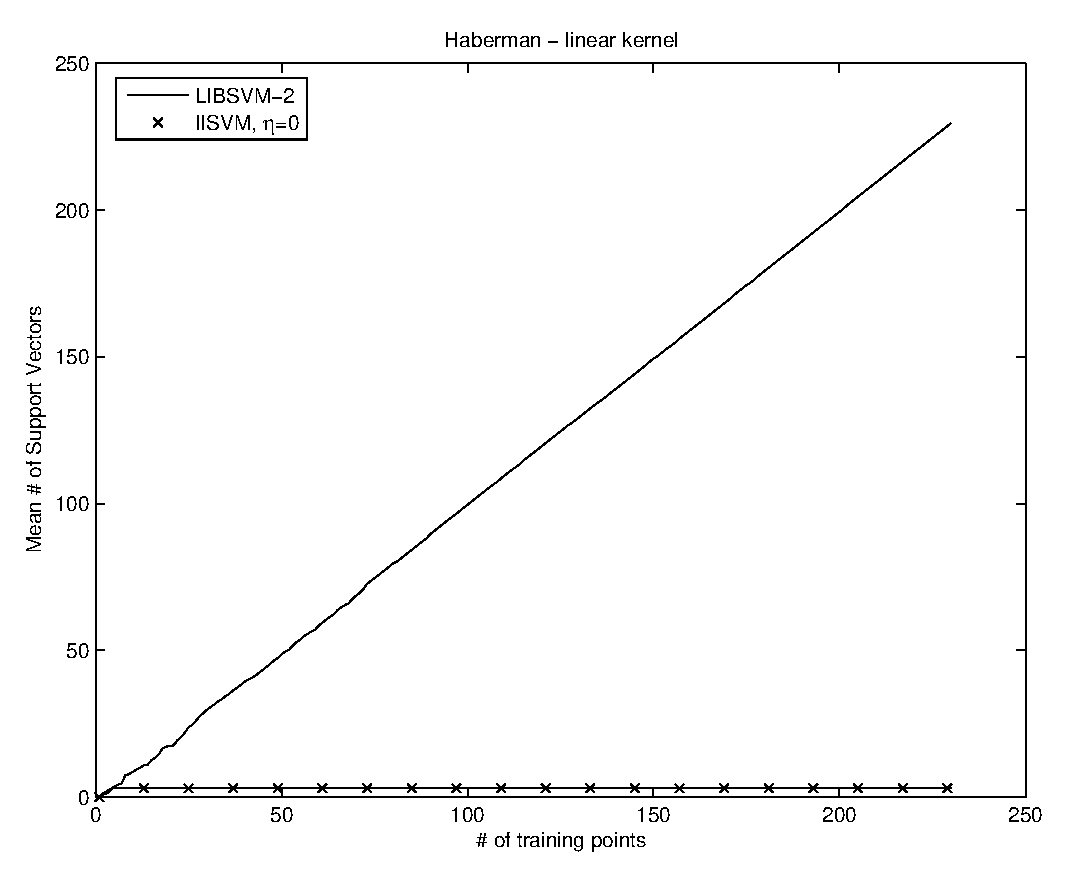
\includegraphics[width=0.45\textwidth]{Haberman_lin} &
       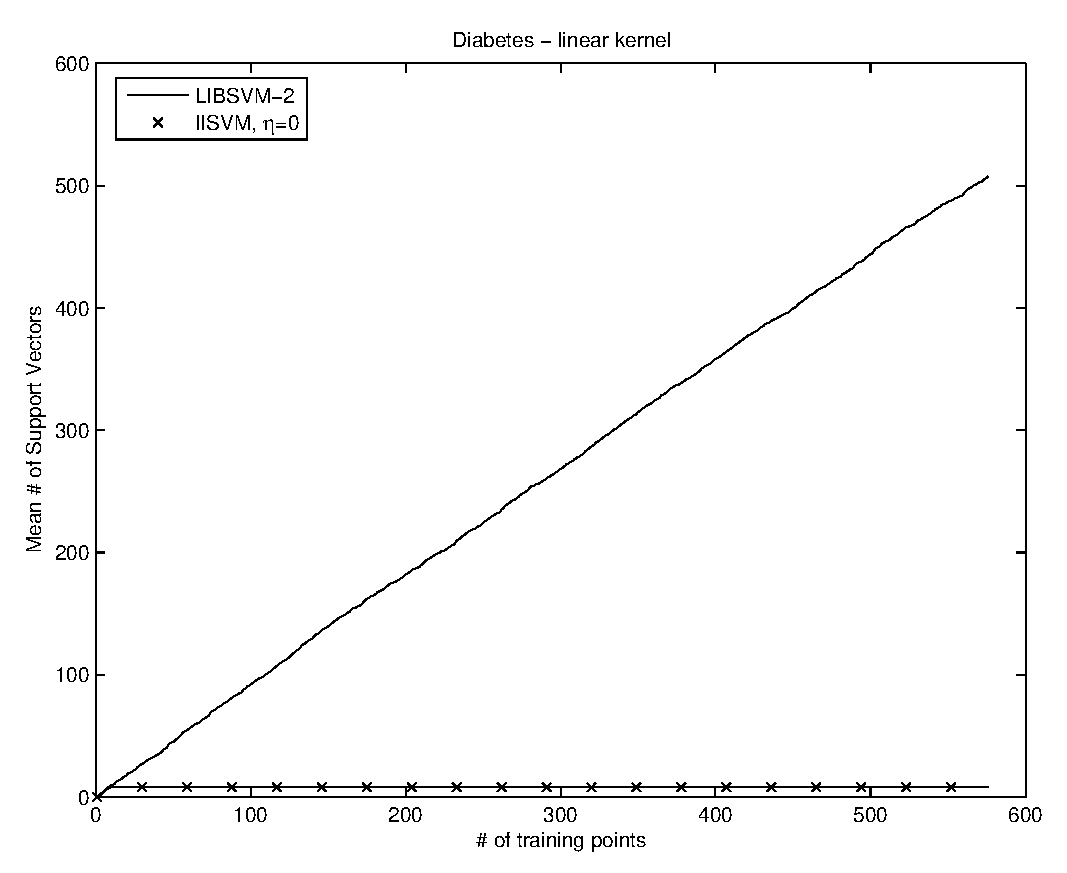
\includegraphics[width=0.45\textwidth]{Diabetes_lin} \\
       \multicolumn{2}{c}{(a)} \\
       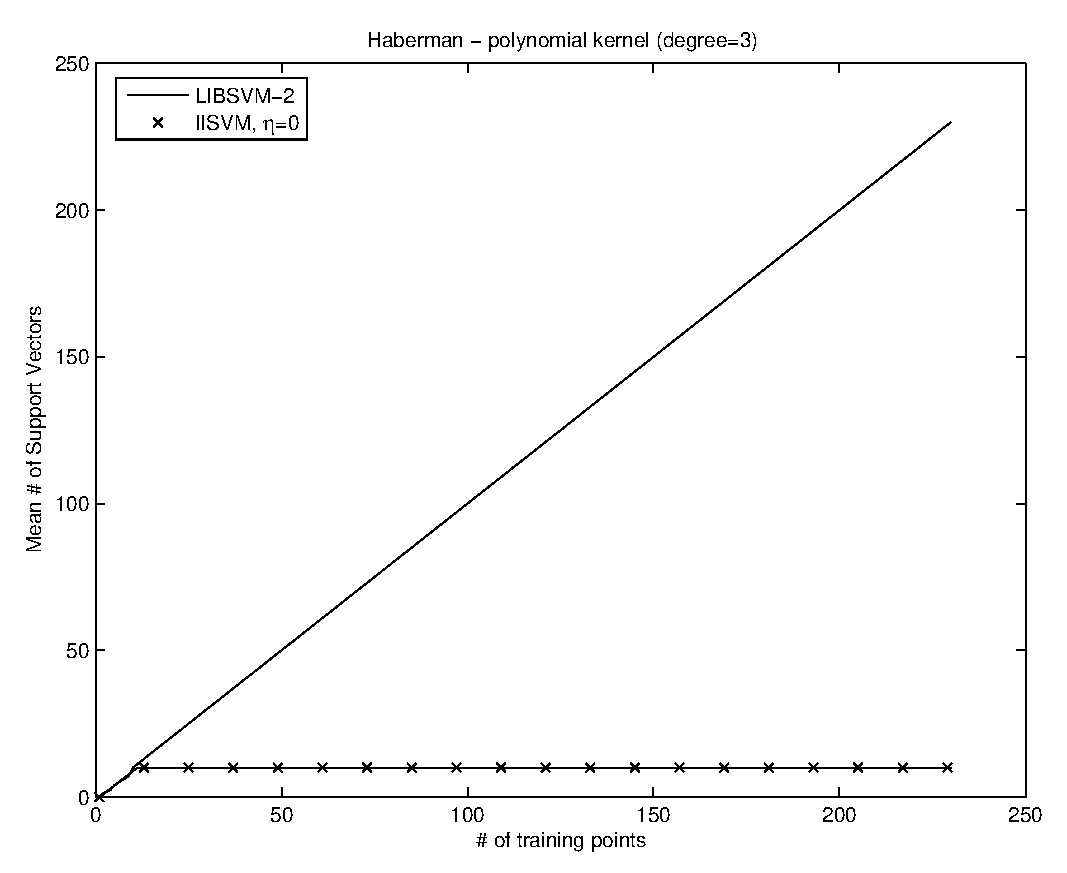
\includegraphics[width=0.45\textwidth]{Haberman_poly3} &
       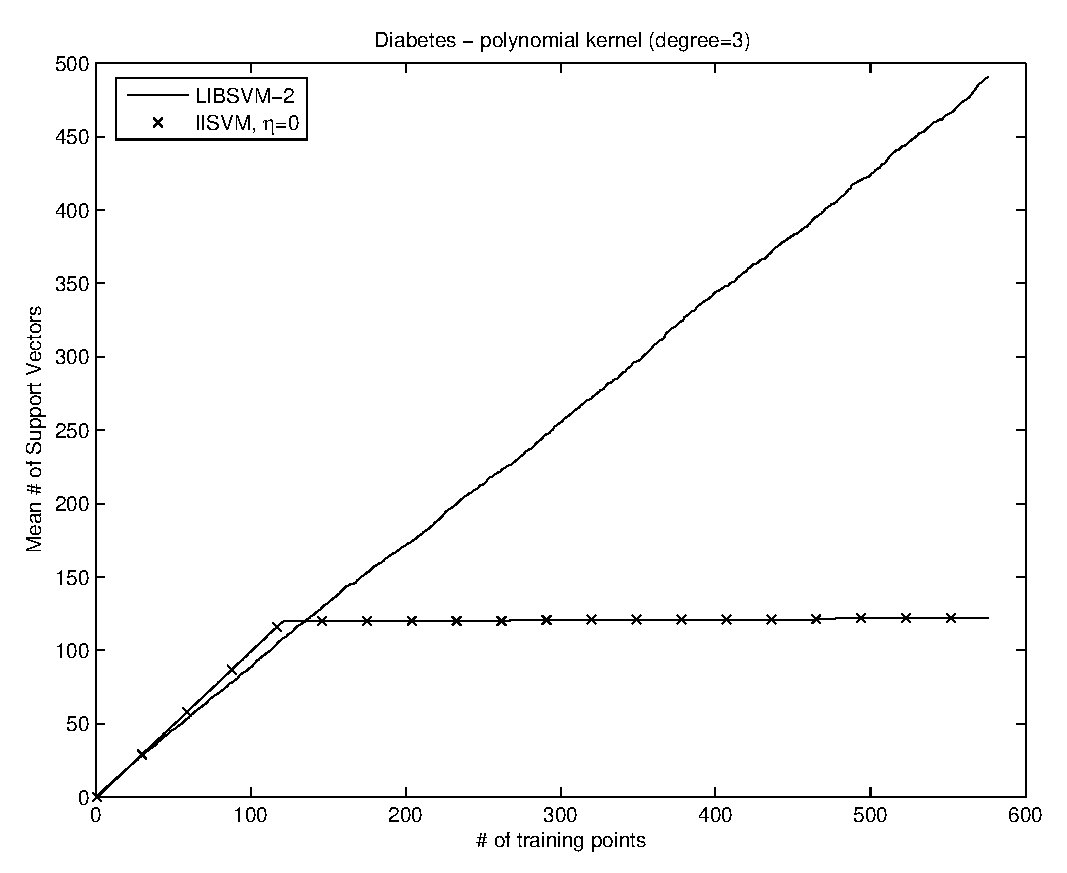
\includegraphics[width=0.45\textwidth]{Diabetes_poly3} \\
       \multicolumn{2}{c}{(b)} \\
    \end{tabular}
  \end{center}
  \caption{\label{fig:finite} test results with finite-dimensional
  kernels: (a) linear kernel, (b) polynomial kernel with degree $3$.}
\end{figure*}

\begin{figure*}[!htbp]
  \begin{center}
    \begin{tabular}{cc}
       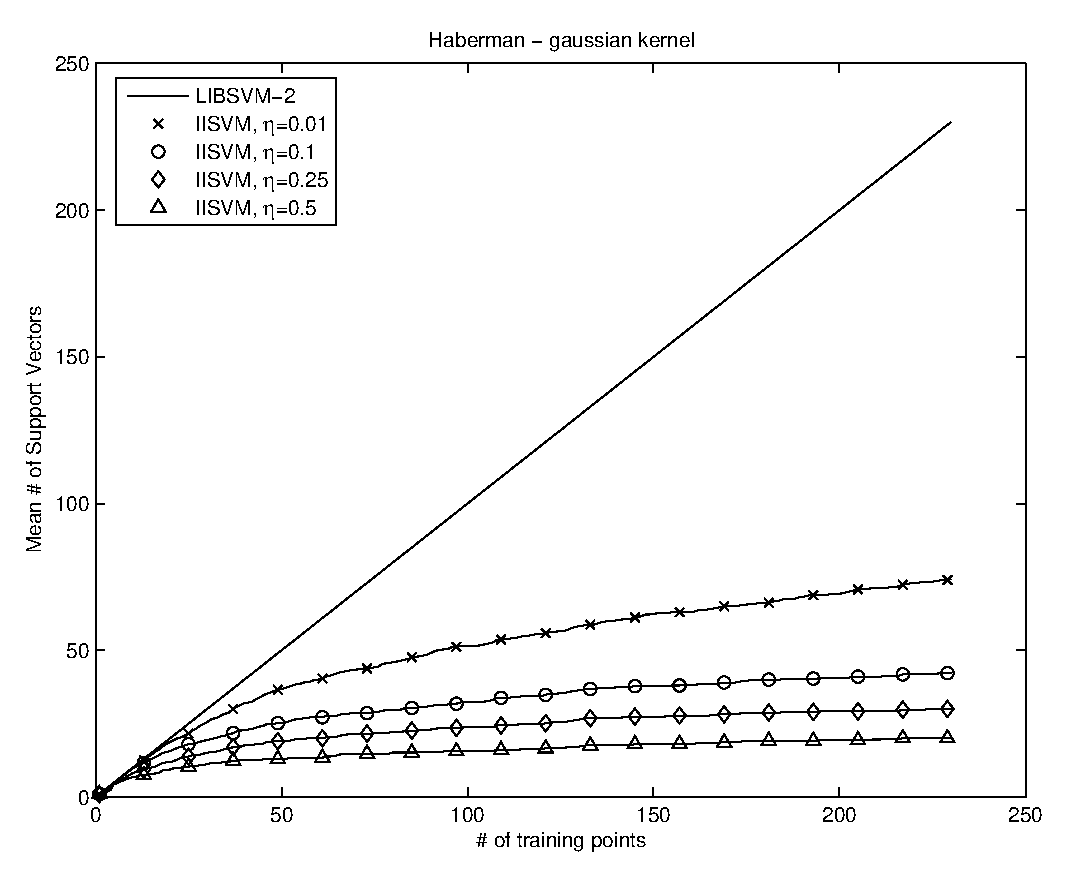
\includegraphics[width=0.45\textwidth]{Haberman_gaussian} &
       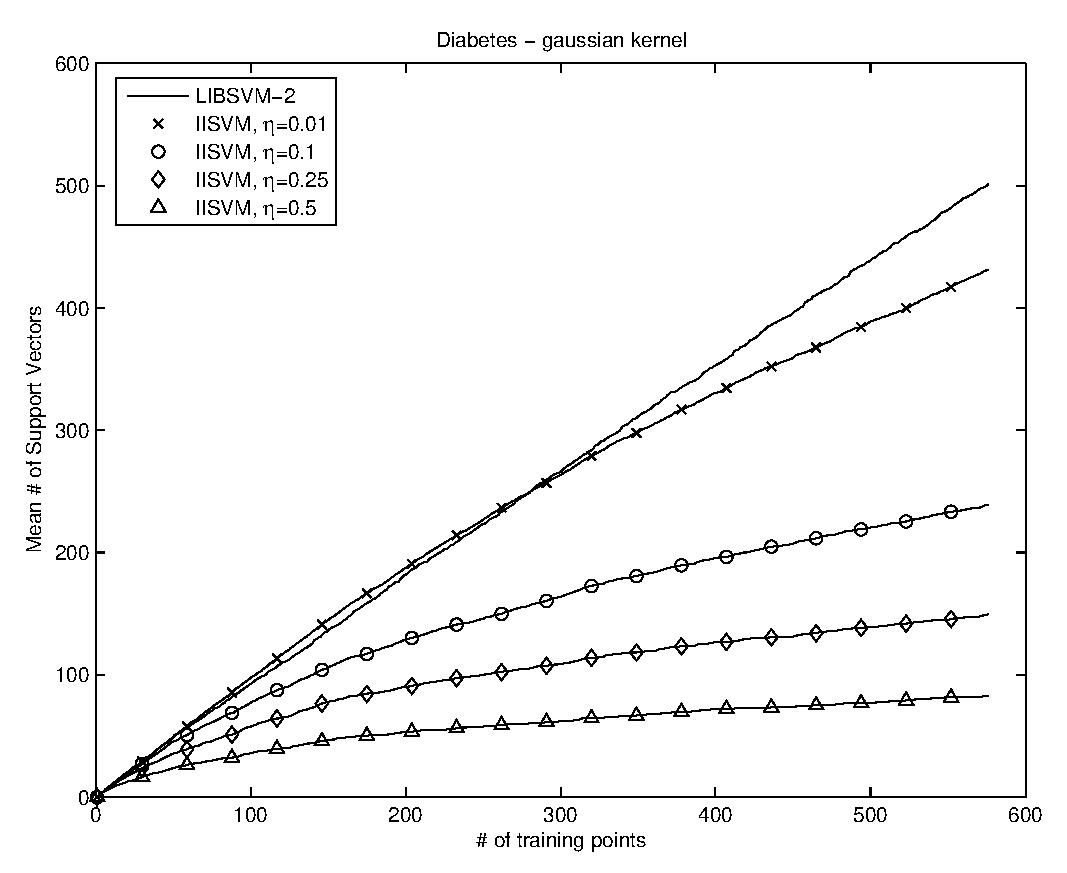
\includegraphics[width=0.45\textwidth]{Diabetes_gaussian}
    \end{tabular}
  \end{center}
  \caption{\label{fig:infinite} test results with an infinite-dimensional
  (Gaussian) kernel.}
\end{figure*}

Consider Figure \ref{fig:finite}: as one can see, as opposed to the
linear behaviour of LIBSVM-2, IISVMs quickly attain a constant number
of support vectors and then stop acquiring new ones. The values are,
in turn, $3$ support vectors in Figure \ref{fig:finite}(a) and $10$
and $120$ in Figure \ref{fig:finite}(b). These numbers match exactly
the dimensions of the related feature spaces, given by
$\binom{m+deg-1}{deg}$ where $deg$ is the degree of the polynomial
kernel (obviously $1$ in the case of linear kernels).

Consider Figure \ref{fig:infinite}: in this case IISVMs obtains a
dramatic reduction in the number of support vectors, as expected, as
the tolerance threshold $\eta$ is made larger and larger. Also, the
shape of the curve seems in most cases to be no longer linear but
rather somehow logarithmic. As $\eta$ is raised, as expected, the
relative error\footnote{let $e$ and $e'$ be the error obtained
in turn by IISVM and LIBSVM-2; then the relative error is defined as
$(e'-e)/e'$.} with respect to LIBSVM-2 grows, but
in a remarkably small way: in the worst cases, that is for $\eta=0.5$,
the relative error is slightly more than $1\%$ with respect to
LIBSVM-2, whereas it is $0.24\%$ for the Haberman suite.

As a final remark, notice that in general the number of support
vectors chosen by IISVMs could be higher than that obtained by
SVMs. An example of this phenomenon is visible in Figure
\ref{fig:infinite}, right plot, between x-values $100$ and $200$.

\section{Conclusions}
\label{sec:concl}

A new method is presented to keep Support Vector Machines small,
called IISVMs (Incremental Independent Support Vector
Machines). IISVMs avoid inserting into their kernel matrix support
vectors which are linearly dependent of previous ones in the feature
space --- in other words, the kernel matrix is always kept at full
rank. The primal SVM problem is then solved via an incremental
algorithm which benefits of the small size of the kernel matrix.

Experimental results show that $(i)$ in the case of finite-dimensional
kernels, IISVMs attain the theoretical limit of linearly independent
support vectors allowed by the feature space; $(ii)$ in the case of
infinite-dimensional kernels, they dramatically reduce the number
support vectors at the price of a negligible degradation in the
accuracy. Notice that, in this latter case also, they can be used to
obtain full precision, choosing the tolerance threshold to be equal to
machine precision.

Besides extending the approach to the problem of regression, future
work is mainly developing in two directions: first, toward a
theoretical characterisation of the results presented above; second,
toward a fast implementation of IISVM in an online environment for
object recognition, robotic kinematic models and grasping.

% ------------------------------------------------------------------------ 

{\small
\bibliographystyle{ieee}
\bibliography{paper}
}

\end{document}
